\documentclass{article}
\usepackage{graphicx} % Required for including images
\usepackage{booktabs} % Required for better horizontal rules in tables
\usepackage{amsmath} % Required for math features
\usepackage[margin=1in]{geometry} % Set margins
\usepackage{hyperref} % For hyperlinks in the PDF
\usepackage{multicol} % For multiple columns
\usepackage{float} % Required for the 'H' float option
\geometry{
 a4paper,
 left=20mm,
 top=20mm,
}

\title{Codebase: GLMC}
\author{Harry}
\date{Last Update: \today}

\begin{document}

\maketitle

\begin{multicols}{2} % Start a two-column layout
% Left column
\section{2023/11/13 CE Loss}
\begin{table}[H]
\centering
\caption{Experiment Parameters}
\label{tab:parameters}
\begin{tabular}{ll}
\toprule
Parameter & Value \\
\midrule
Dataset & CIFAR-10 \\
Architecture & ResNet-32 \\
Loss & CE \\
Number of Classes & 10 \\
Imbalance Rate & 0.01 \\
Learning Rate & 0.01 \\
Epochs & 200 \\
Batch Size & 64 \\
Momentum & 0.9 \\
Weight Decay & 0.005 \\
knn & False/True \\
% Include other parameters as needed
\bottomrule
\end{tabular}
\end{table}

\textbf{Results Summary}:
\begin{itemize}
    \item Training Time: 45 min 58.60 sec (1:00:15.68 with knn)
    \item Per class num: [5000, 2997, 1796, 1077, 645, 387, 232, 139, 83, 50]
    \item Best Precision@1: 78.27\%  (83.1\% with knn)
    \item Final Epoch Loss: 0.0080 (0.0085 with knn)
    \item Validation Precision@1: 77.19\% (82.390\% with knn)
    \item Validation Precision@5: 97.98\% (99.120\% with knn)
\end{itemize}

% Right column
\columnbreak
\begin{figure}[H]
\centering
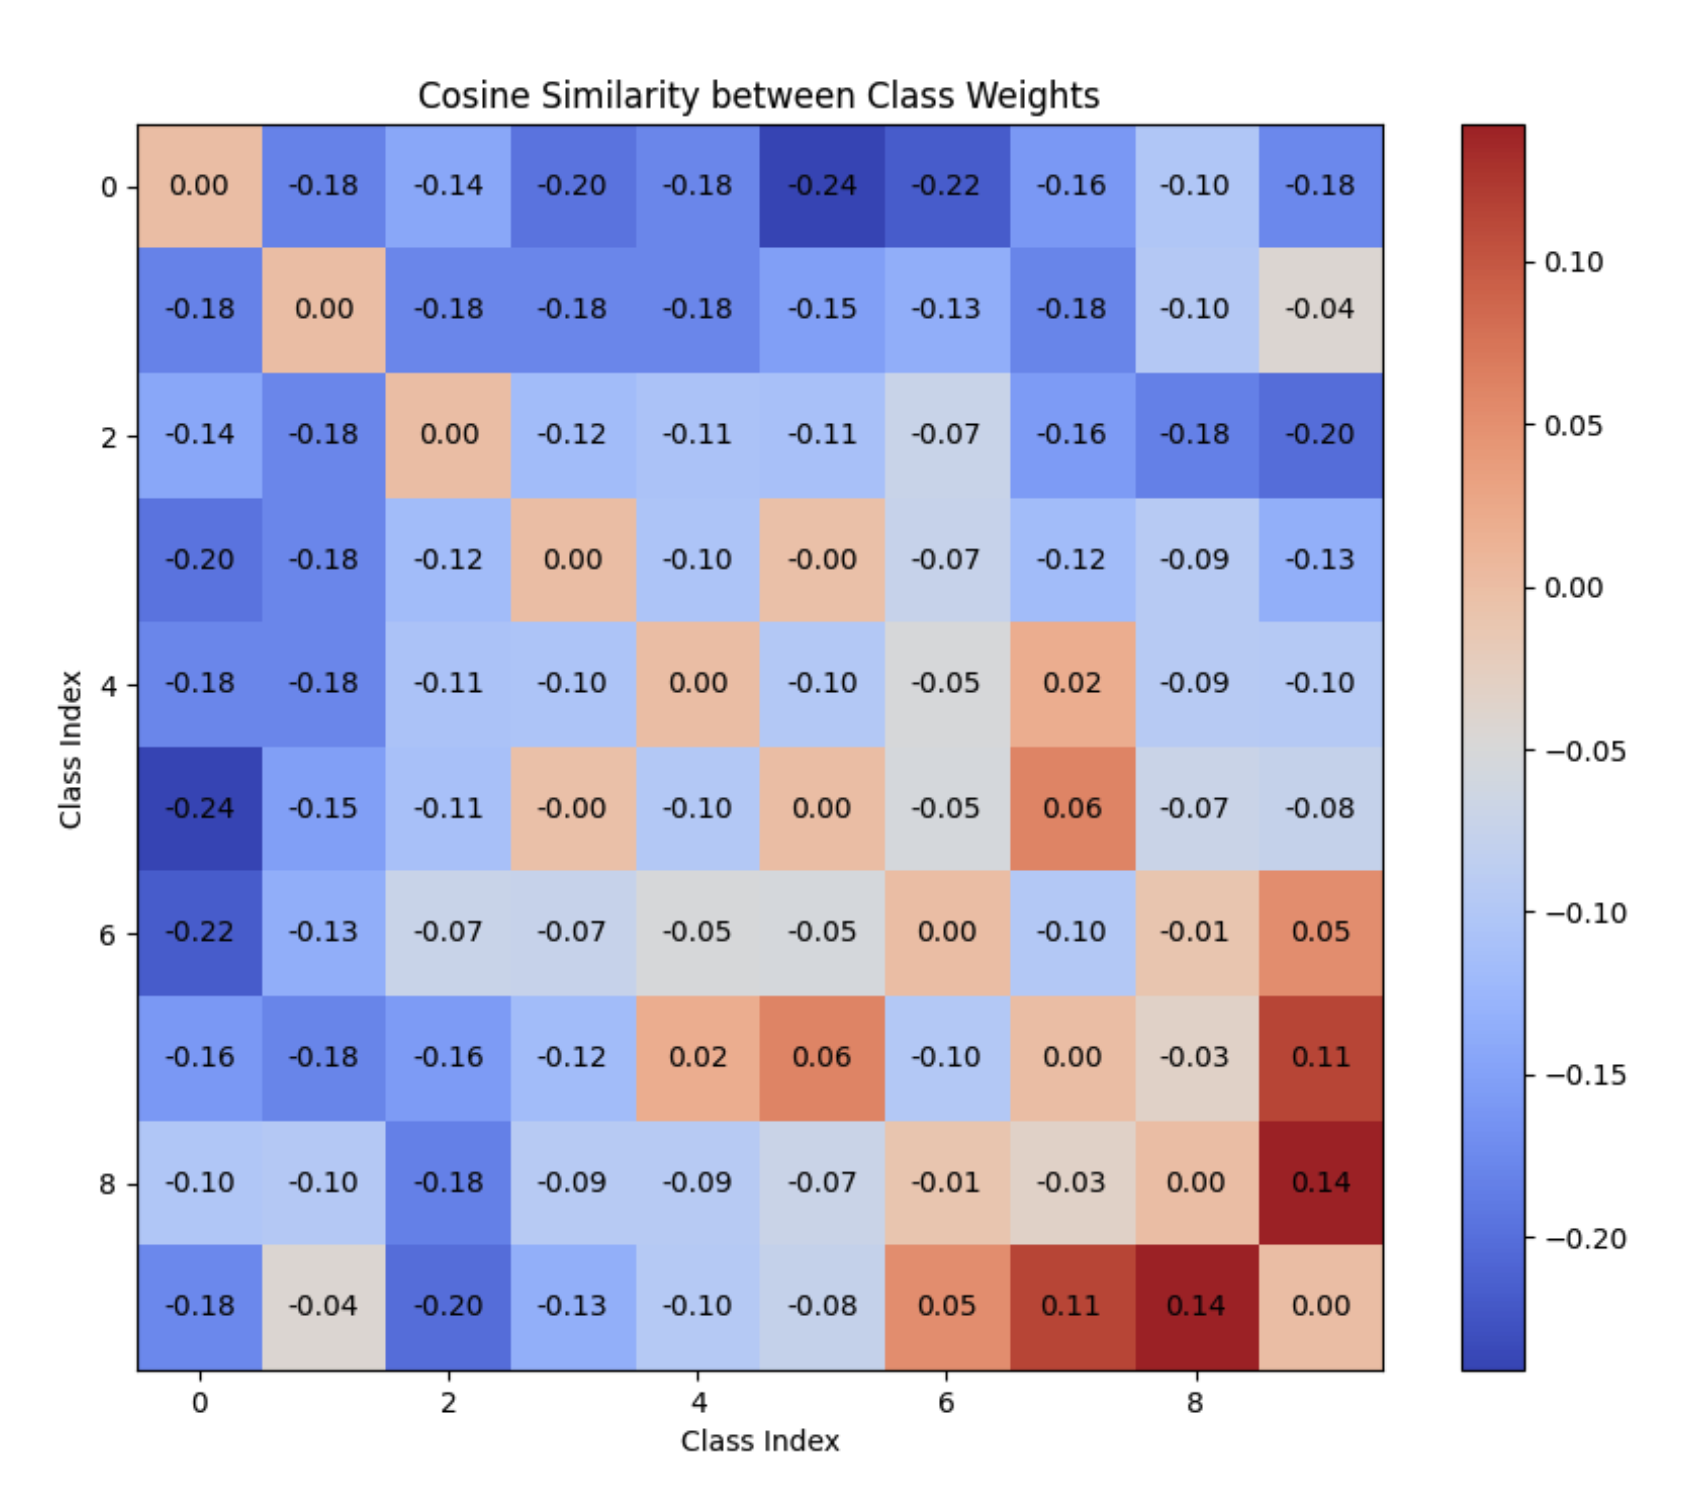
\includegraphics[width=\linewidth]{Plot/CE/cosine_similarity_between_class_weights.png}
\caption{Cosine Similarity between Class Weights}
\end{figure}
\begin{figure}[H]
\centering
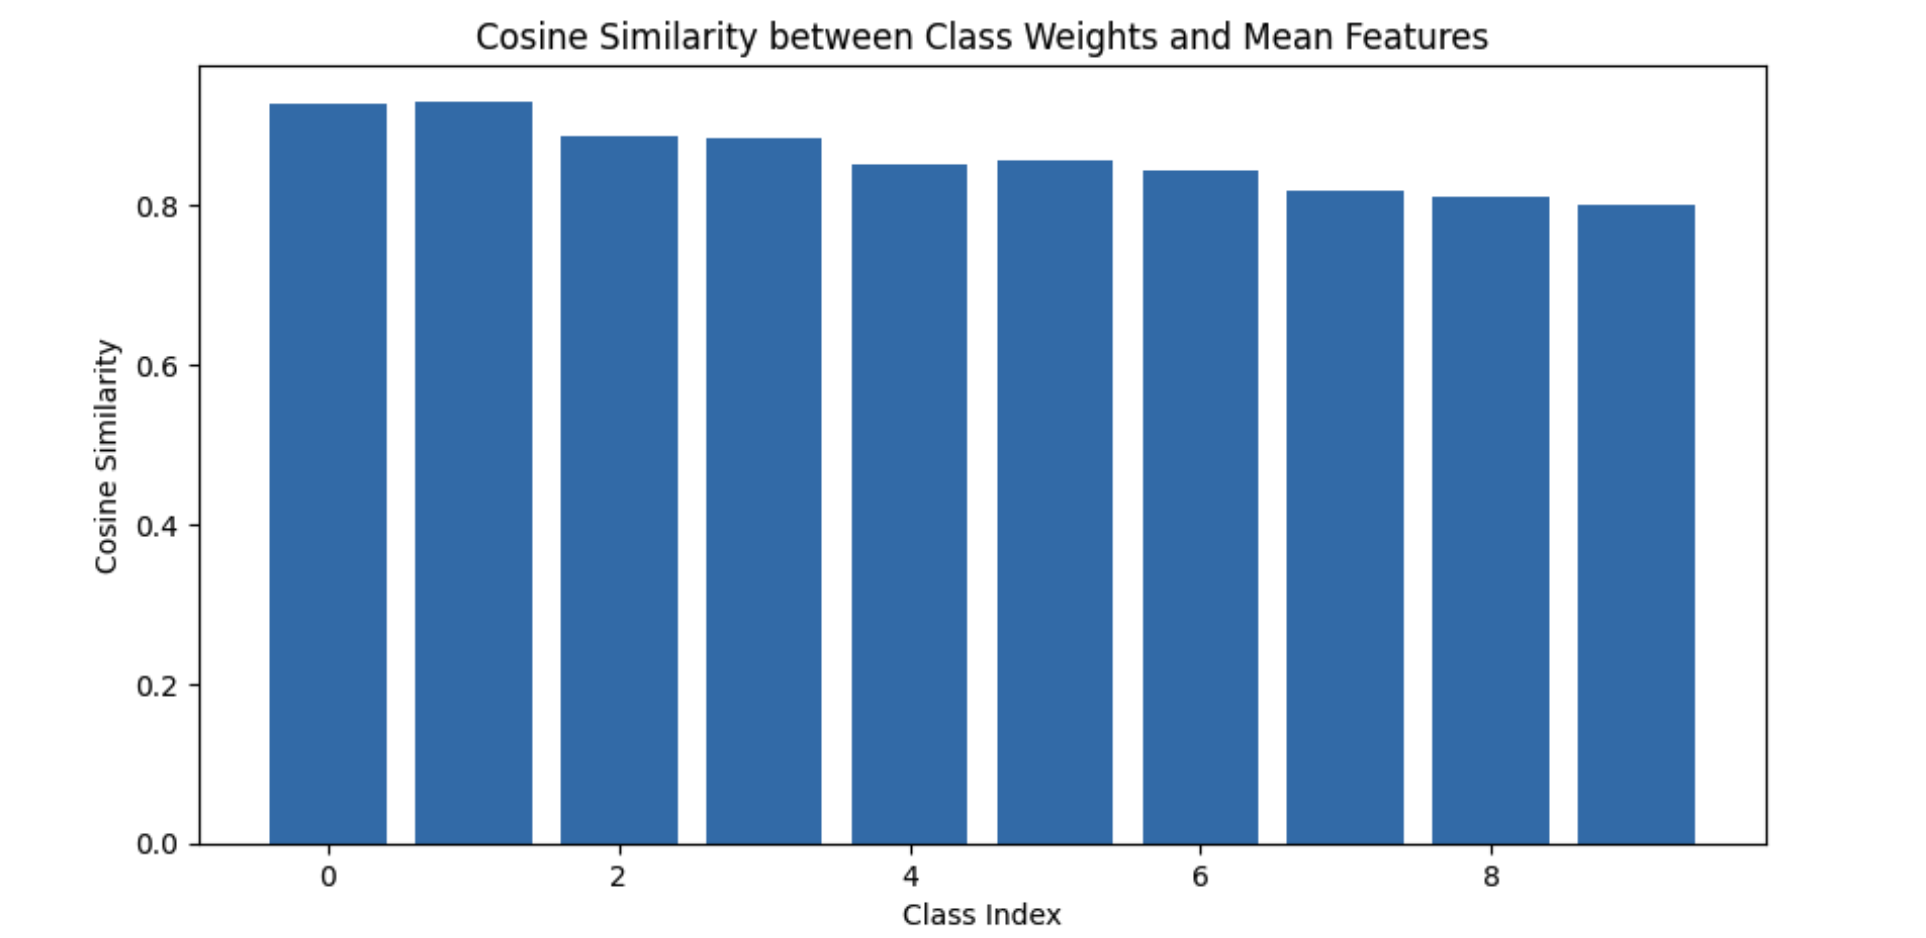
\includegraphics[width=\linewidth]{Plot/CE/cosine_similarity_between_class_weights_and_mean_features.png}
\caption{Cosine Similarity between Class Weights and Mean Features}
\end{figure}

\end{multicols} % End the two-column layout



\newpage

\begin{multicols}{2} % Start a two-column layout
% Left column
\section{2023/11/15 VS Loss}
\begin{table}[H]
\centering
\caption{Experiment Parameters}
\label{tab:parameters_vs}
\begin{tabular}{ll}
\toprule
Parameter & Value \\
\midrule
Dataset & CIFAR-10 \\
Architecture & ResNet-32 \\
Loss & VS \\
Number of Classes & 10 \\
Imbalance Rate & 0.01 \\
Learning Rate & 0.01 \\
Epochs & 200 \\
Batch Size & 64 \\
Momentum & 0.9 \\
Weight Decay & 0.005 \\
knn & False\\
\(\gamma\) & 0.15 \\
\(\tau\) & 1.25 \\
% Include other parameters as needed
\bottomrule
\end{tabular}
\end{table}

\textbf{Results Summary}:
\begin{itemize}
    \item Training Time: 45 min 46.36 sec
    \item Per class num: [5000, 2997, 1796, 1077, 645, 387, 232, 139, 83, 50]
    \item Best Precision@1: 82.080\%
    \item Final Epoch Loss: 0.0183
    \item Validation Precision@1: 81.840\%
    \item Validation Precision@5: 97.160\%
\end{itemize}

% Right column
\columnbreak
\begin{figure}[H]
\centering
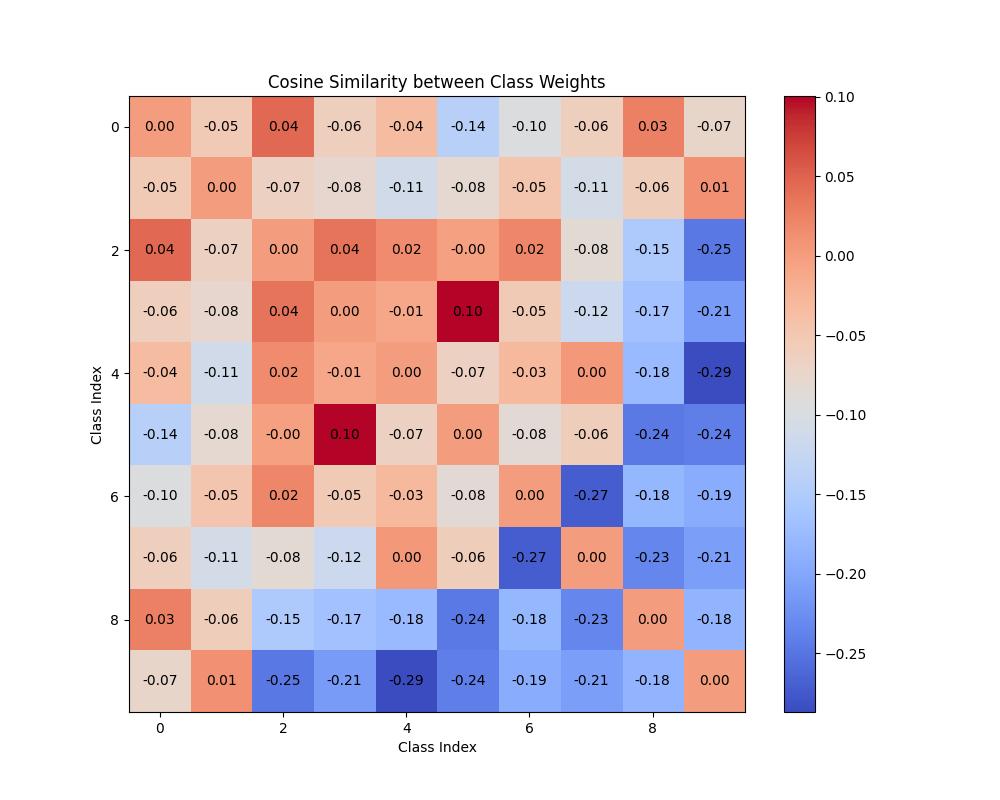
\includegraphics[width=\linewidth]{Plot/VS/VS_cos_190_gm015_tau125.png}
\caption{Cosine Similarity between Class Weights}
\end{figure}
\begin{figure}[H]
\centering
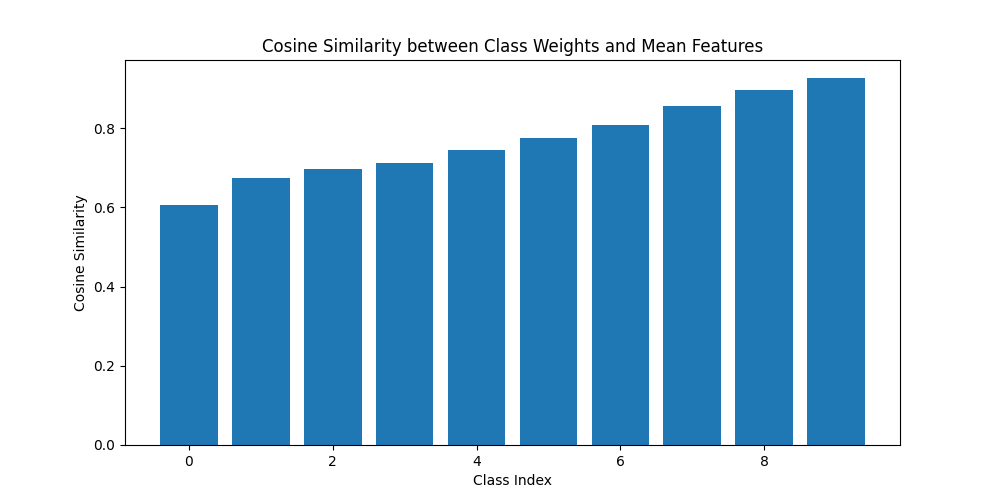
\includegraphics[width=\linewidth]{Plot/VS/VS_WiHi_190_gm015_tau125.png}
\caption{Cosine Similarity between Class Weights and Mean Features}
\end{figure}

\end{multicols} % End the two-column layout





\newpage

\begin{multicols}{2} % 开始两栏布局
% 左栏
\section{2023/11/20 VS Loss}
\begin{table}[H]
\centering
\caption{Experiment Parameters}
\label{tab:parameters_vs}
\begin{tabular}{ll}
\toprule
Parameter & Value \\
\midrule
Dataset & CIFAR-10 \\
Architecture & ResNet-50 \\
Number of Classes & 10 \\
Loss & VS \\
Imbalance Rate & 0.01 \\
Learning Rate & 0.01 \\
Epochs & 200 \\
Batch Size & 64 \\
Momentum & 0.9 \\
Weight Decay & 0.005 \\
knn & True \\
\(\gamma\) & 0.15 \\
\(\tau\) & 1.25 \\
% Include other parameters as needed
\bottomrule
\end{tabular}
\end{table}

\textbf{Results Summary}:
\begin{itemize}
    \item Training Time: 91 min 36.66 sec
    \item Per class num: [5000, 2997, 1796, 1077, 645, 387, 232, 139, 83, 50]
    \item Best Precision@1: 75.160\%
    \item Final Epoch Loss: 0.0689
    \item Validation Precision@1: 74.770\%
    \item Validation Precision@5: 97.540\%
\end{itemize}

% 右栏
\columnbreak
\begin{figure}[H]
\centering
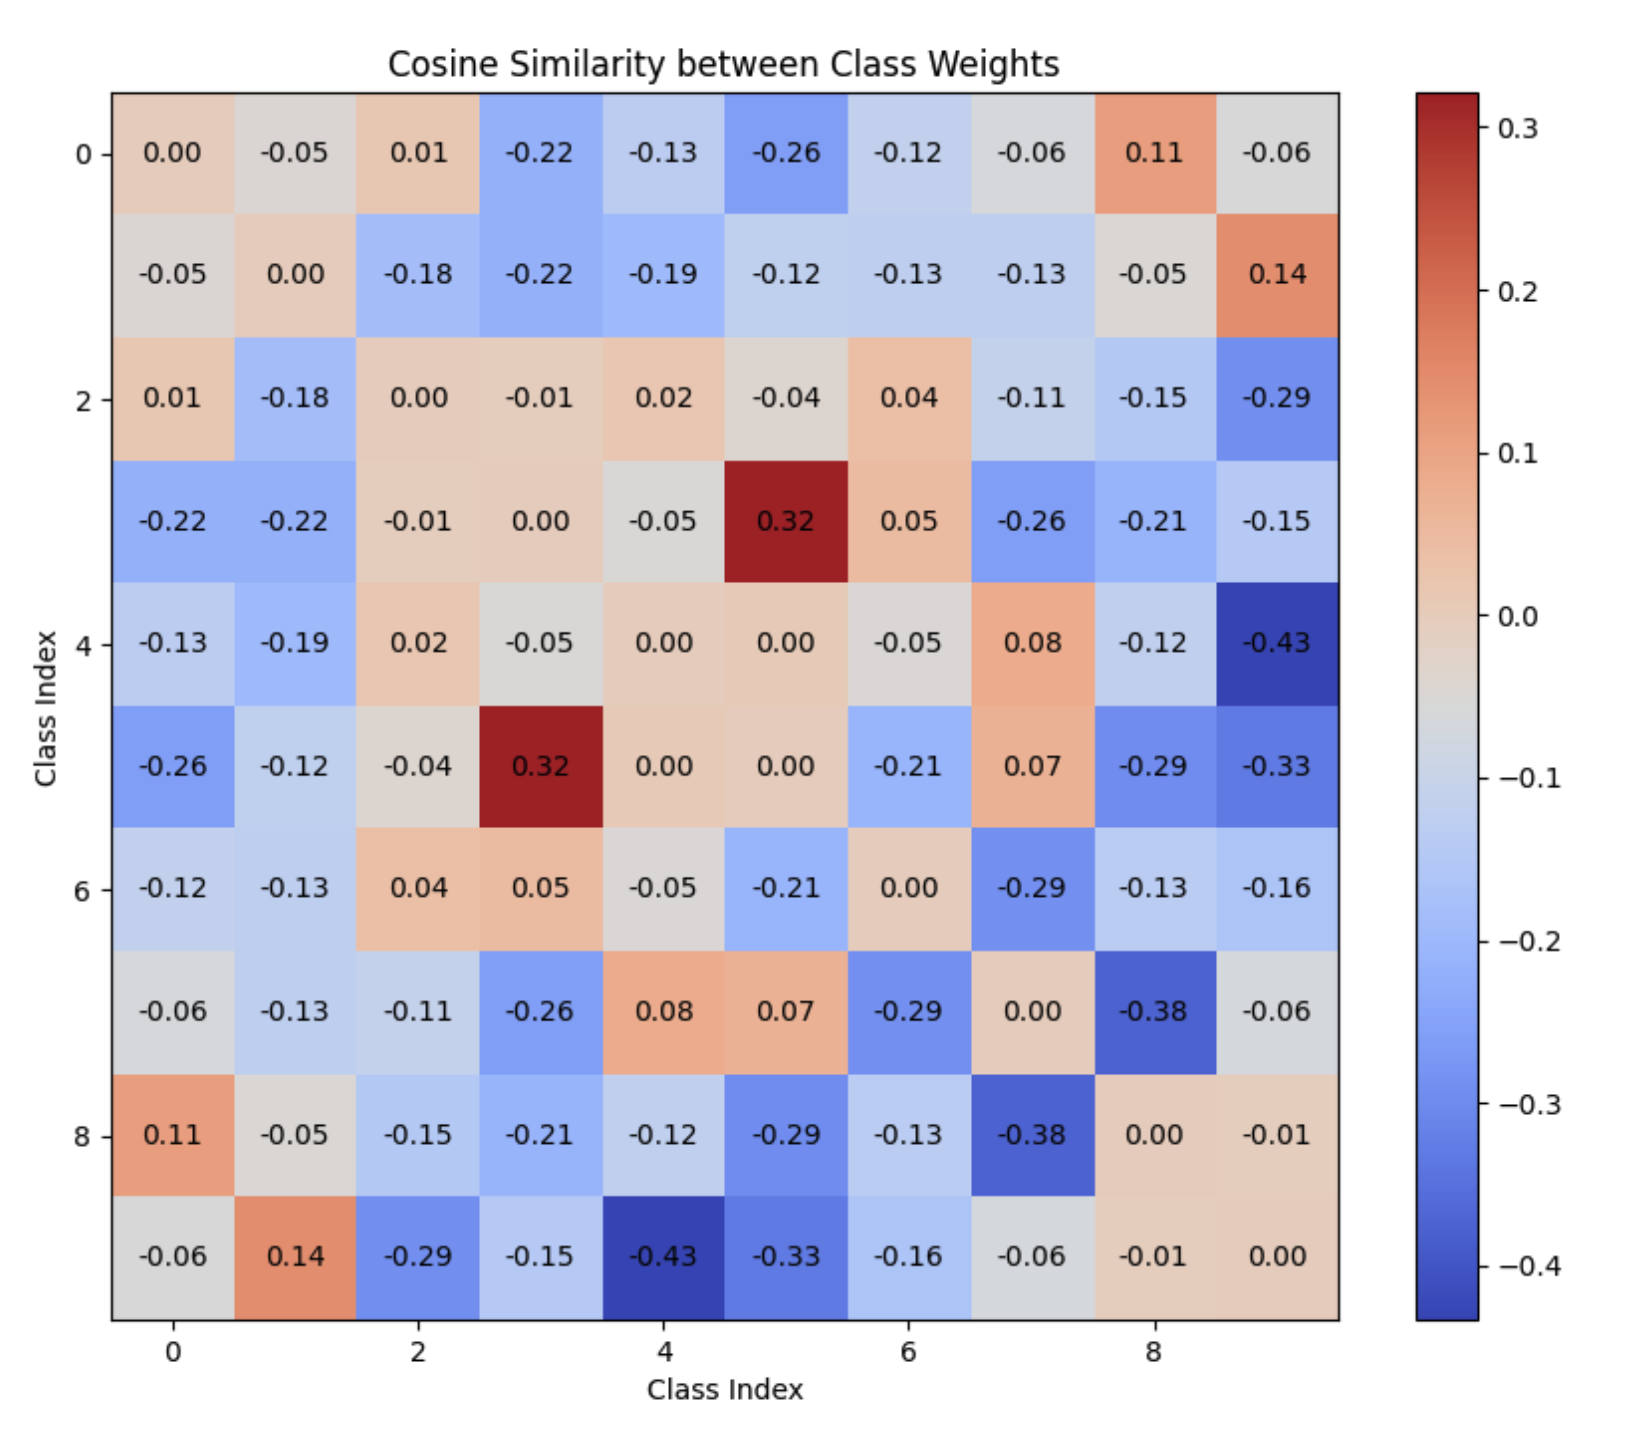
\includegraphics[width=\linewidth]{Plot/VS_res50/cos_res50.png}
\caption{Cosine Similarity between Class Weights}
\end{figure}
\begin{figure}[H]
\centering
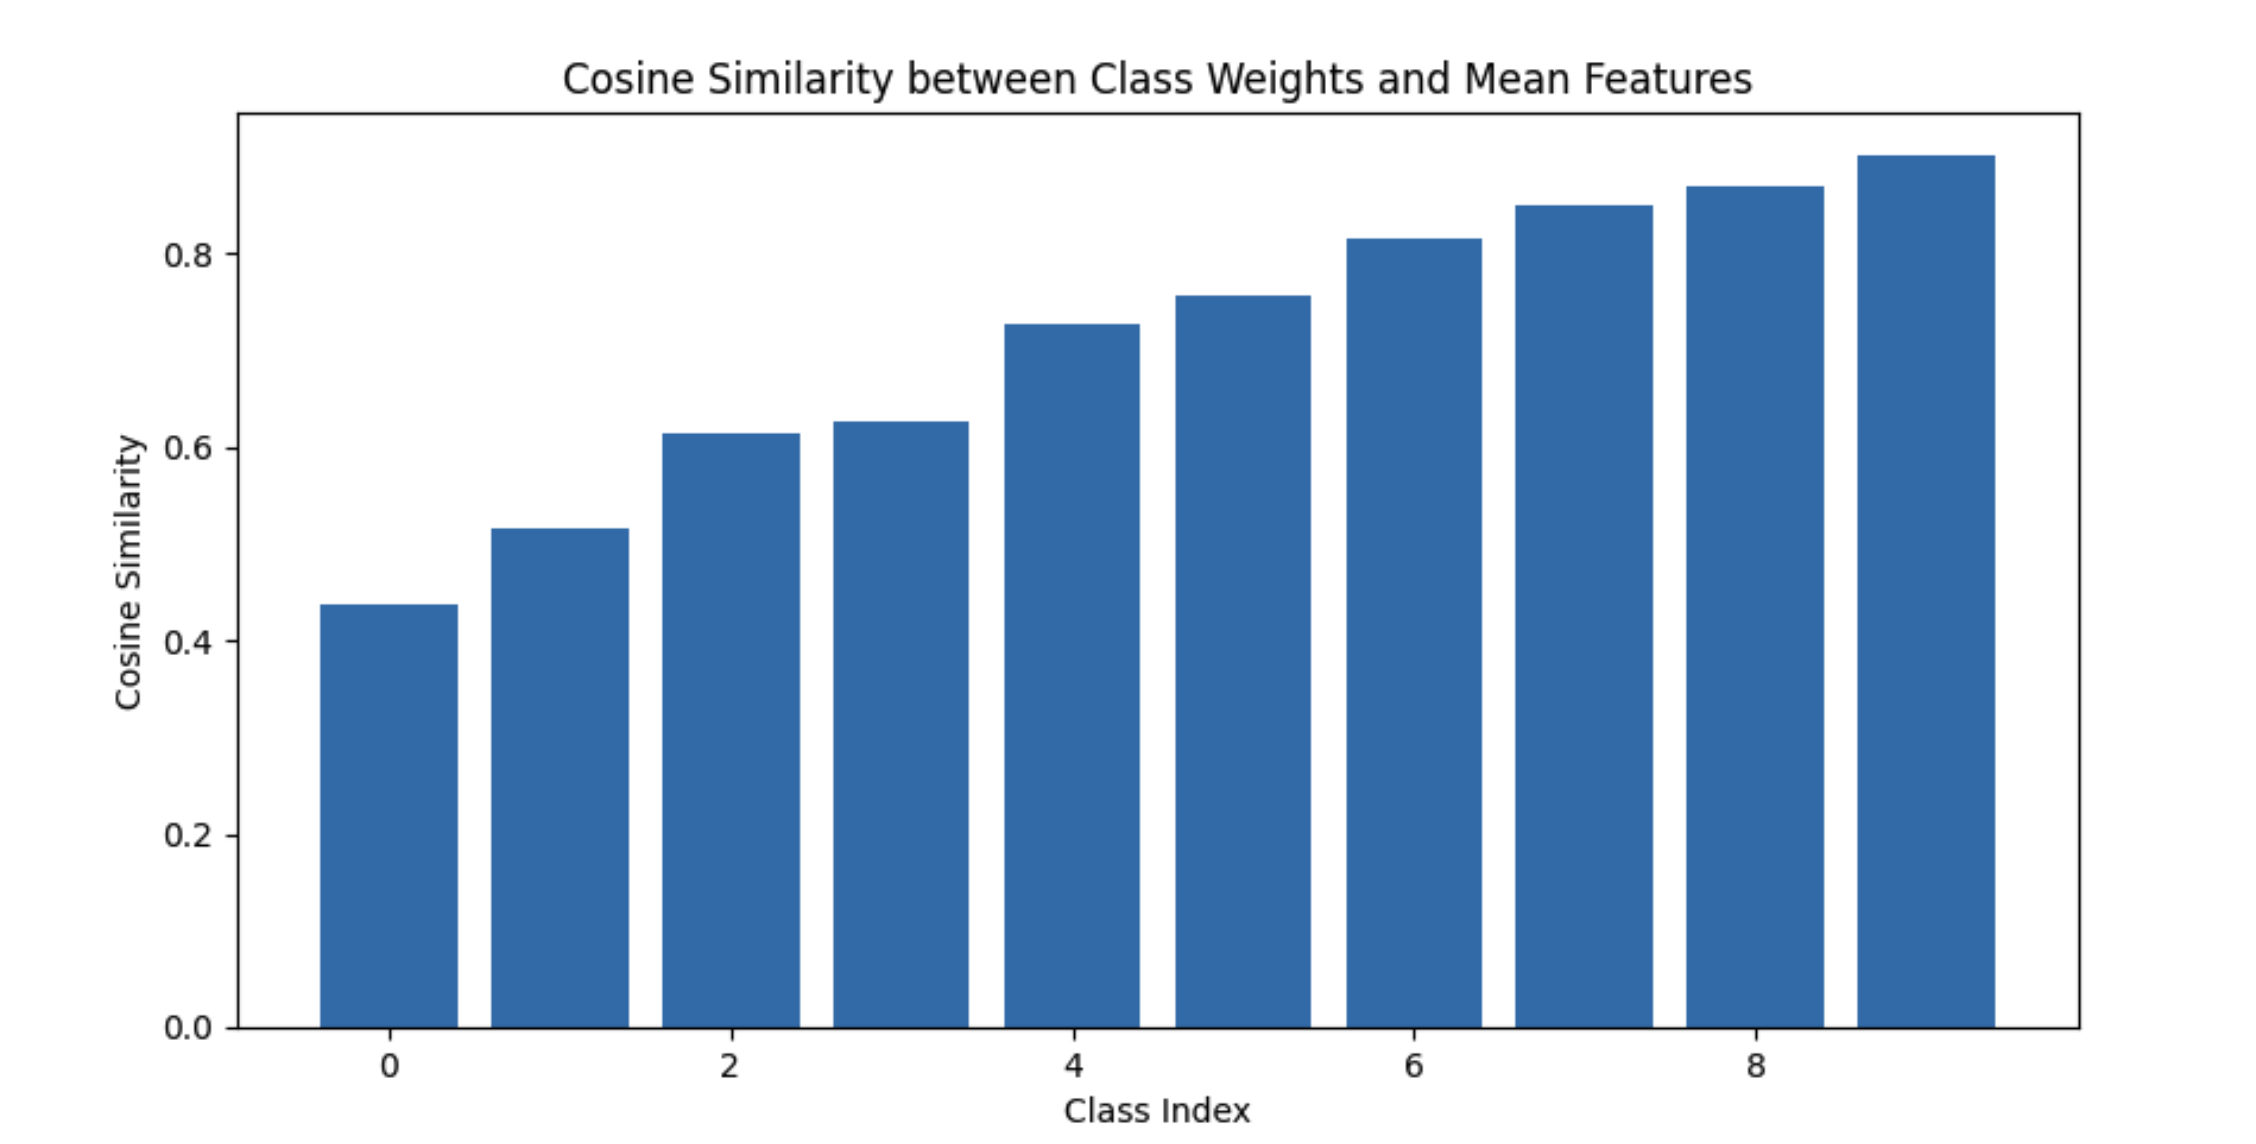
\includegraphics[width=\linewidth]{Plot/VS_res50/Wi_Hi_res50.png}
\caption{Cosine Similarity between Class Weights and Mean Features}
\end{figure}

\end{multicols} % 结束两栏布局





\newpage

\begin{multicols}{2} % 开始两栏布局
% 左栏
\section{2023/11/21 CE Loss stage --1}
\begin{table}[H]
\centering
\caption{Experiment Parameters}
\label{tab:parameters}
\begin{tabular}{ll}
\toprule
Parameter & Value \\
\midrule
Dataset & CIFAR-10 \\
Architecture & ResNet-32 \\
Loss & CE \\
Number of Classes & 10 \\
Imbalance Rate & 0.01 \\
Learning Rate & 0.01 \\
Epochs & 200 \\
Batch Size & 64 \\
Momentum & 0.9 \\
Weight Decay & 0.005 \\
knn & True \\
% Include other parameters as needed
\bottomrule
\end{tabular}
\end{table}

\textbf{Results Summary}:
\begin{itemize}
    \item Training Time: 57 min 34 sec
    \item Per class num: [5000, 5000, 5000, 5000, 5000, 50, 50, 50, 50, 50]
    \item Best Precision@1: 70.390\%  
    \item Final Epoch Loss: 0.04 
    \item Validation Precision@1: 66.660\%
    \item Validation Precision@5: 98.810%
\end{itemize}

% 右栏
\columnbreak
\begin{figure}[H]
\centering
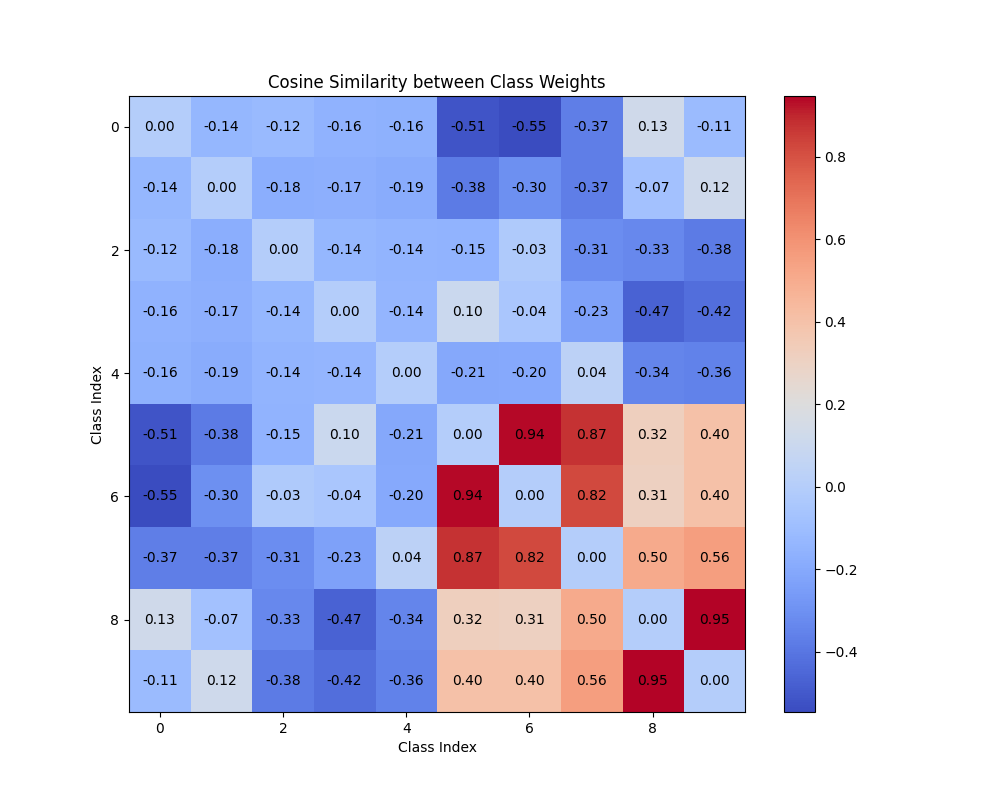
\includegraphics[width=\linewidth]{Plot/CE/stage--1/cos_VS_5000_50_epoch_199.png}
\caption{Cosine Similarity between Class Weights}
\end{figure}
\begin{figure}[H]
\centering
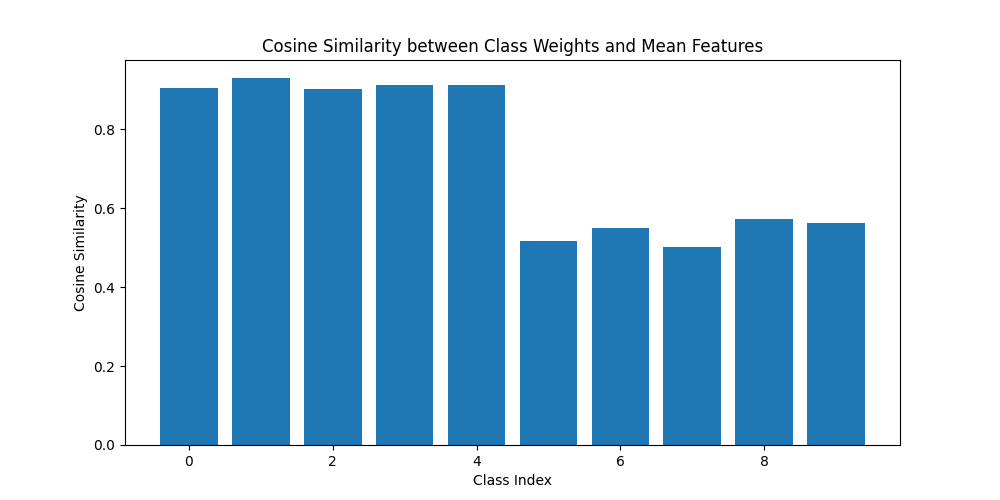
\includegraphics[width=\linewidth]{Plot/CE/stage--1/Wi_Hi_cos_VS_5000_50_epoch_199.png}
\caption{Cosine Similarity between Class Weights and Mean Features}
\end{figure}

\end{multicols} % 结束两栏布局







\newpage

\begin{multicols}{2} % 开始两栏布局
% 左栏
\section{2023/11/21 CE Loss stage --2}
\begin{table}[H]
\centering
\caption{Experiment Parameters}
\label{tab:parameters}
\begin{tabular}{ll}
\toprule
Parameter & Value \\
\midrule
Dataset & CIFAR-10 \\
Architecture & ResNet-32 \\
Loss & CE \\
Number of Classes & 10 \\
Imbalance Rate & 0.01 \\
Learning Rate & 0.01 \\
Epochs & 200 \\
Batch Size & 64 \\
Momentum & 0.9 \\
Weight Decay & 0.005 \\
knn & True \\
% Include other parameters as needed
\bottomrule
\end{tabular}
\end{table}

\textbf{Results Summary}:
\begin{itemize}
    \item Training Time: 57 min 34 sec
    \item Per class num: [5000, 5000, 5000, 50, 50, 50, 50, 50, 50, 50]
    \item Best Precision@1: 65.020\%  
    \item Final Epoch Loss: 0.0182 
    \item Validation Precision@1: 62.860\%
    \item Validation Precision@5: 97.100\%
\end{itemize}

% 右栏
\columnbreak
\begin{figure}[H]
\centering
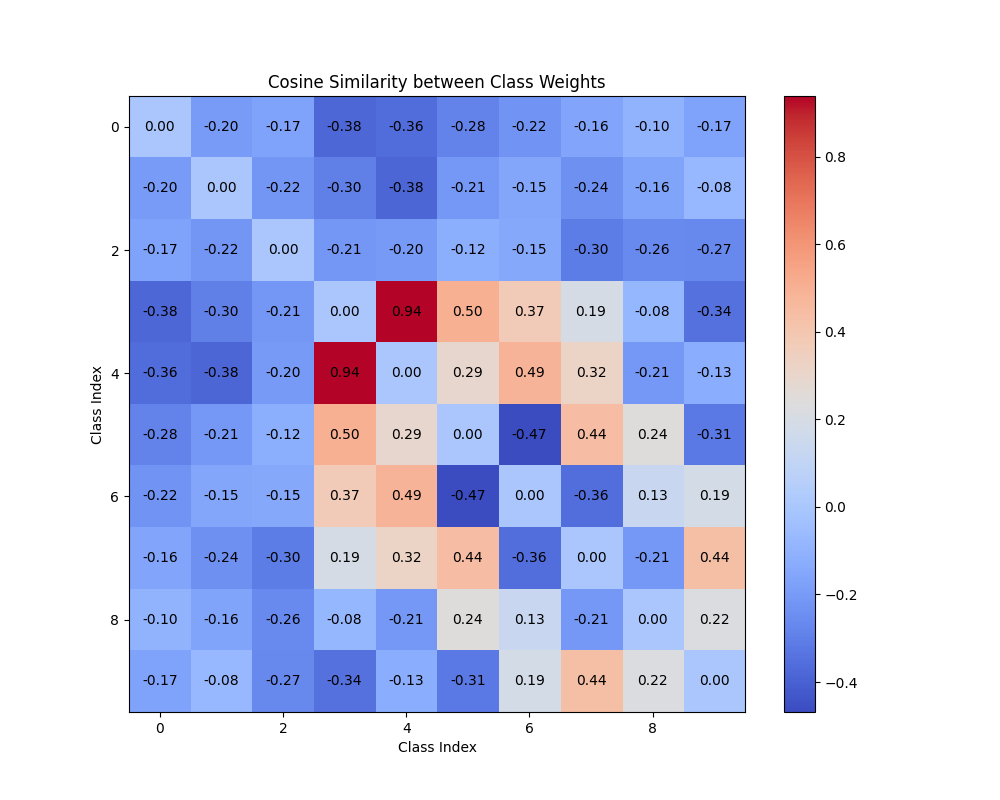
\includegraphics[width=\linewidth]{Plot/CE/stage--2/cos_VS_5000_50_epoch_199.png}
\caption{Cosine Similarity between Class Weights}
\end{figure}
\begin{figure}[H]
\centering
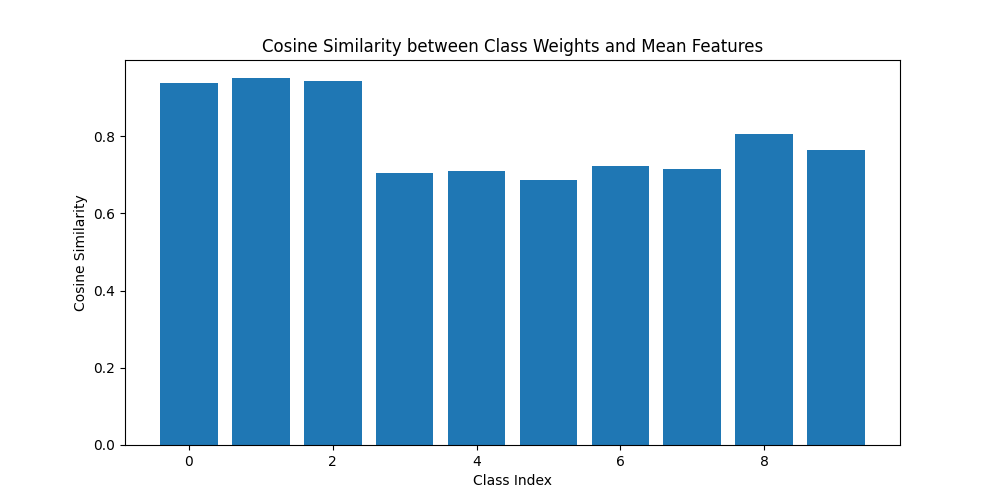
\includegraphics[width=\linewidth]{Plot/CE/stage--2/Wi_Hi_cos_VS_5000_50_epoch_199.png}
\caption{Cosine Similarity between Class Weights and Mean Features}
\end{figure}

\end{multicols} % 结束两栏布局


\newpage

\begin{multicols}{2} % 开始两栏布局
% 左栏
\section{2023/11/21 VS Loss stage}
\begin{table}[H]
\centering
\caption{Experiment Parameters}
\label{tab:parameters}
\begin{tabular}{ll}
\toprule
Parameter & Value \\
\midrule
Dataset & CIFAR-10 \\
Architecture & ResNet-32 \\
Loss & VS \\
Number of Classes & 10 \\
Imbalance Rate & 0.01 \\
Learning Rate & 0.01 \\
Epochs & 200 \\
Batch Size & 64 \\
Momentum & 0.9 \\
Weight Decay & 0.005 \\
\(\gamma\) & 0.15 \\
\(\tau\) & 1.25 \\
knn & True \\
% Include other parameters as needed
\bottomrule
\end{tabular}
\end{table}

\textbf{Results Summary}:
\begin{itemize}
    \item Training Time: 89 min 44 sec
    \item Per class num: [5000, 5000, 5000, 5000, 5000, 50, 50, 50, 50, 50]
    \item Best Precision@1: 75.670\%  
    \item Final Epoch Loss: 0.0446
    \item Validation Precision@1: 74.600\%
    \item Validation Precision@5: 97.550\%
\end{itemize}

% 右栏
\columnbreak
\begin{figure}[H]
\centering
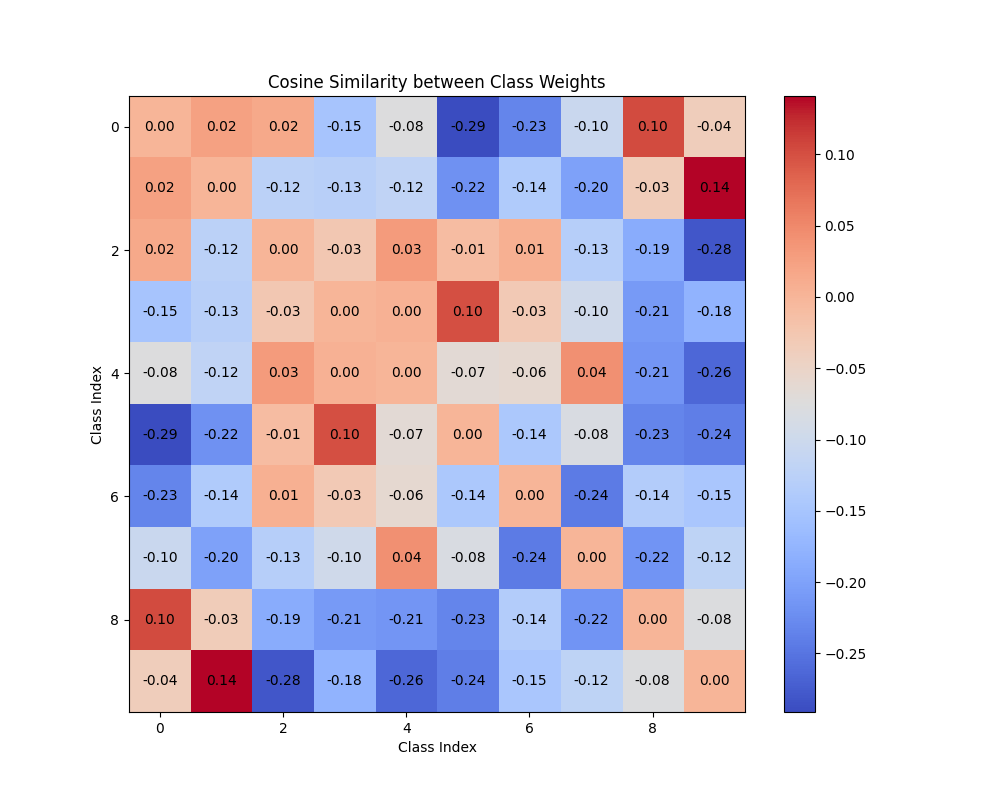
\includegraphics[width=\linewidth]{Plot/VS/stage/cos_VS_5000_50_epoch_199.png}
\caption{Cosine Similarity between Class Weights}
\end{figure}
\begin{figure}[H]
\centering
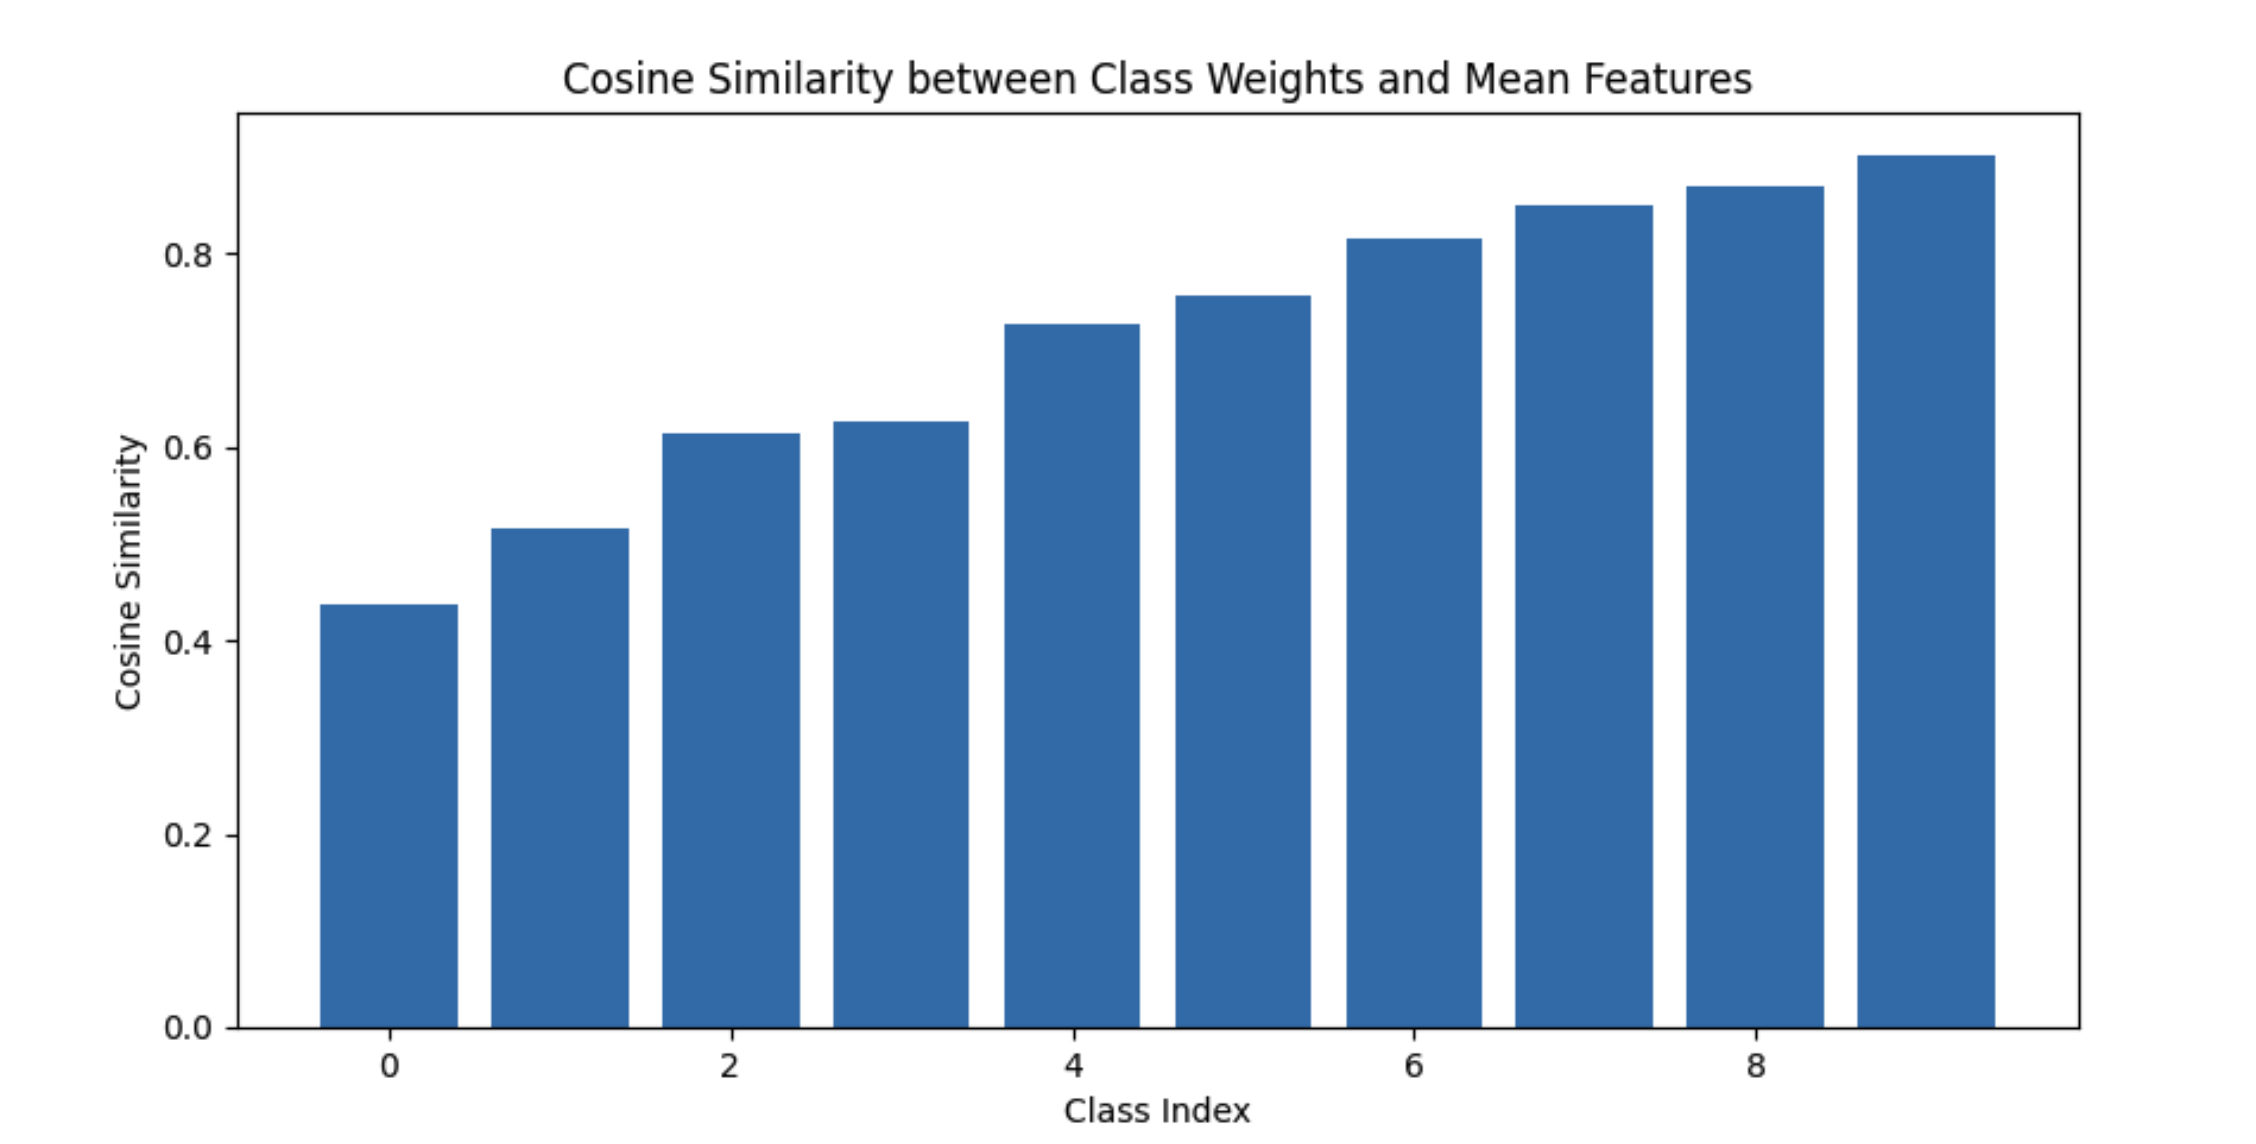
\includegraphics[width=\linewidth]{Plot/VS_res50/Wi_Hi_res50.png}
\caption{Cosine Similarity between Class Weights and Mean Features}
\end{figure}

\end{multicols} % 结束两栏布局



\end{document}
